\documentclass[11pt,a4paper]{jsarticle}

\usepackage{newcent} 
\usepackage[dvipdfm]{graphicx}
\usepackage{comment}
\usepackage{multirow}

\usepackage[dvipdfm,setpagesize=false]{hyperref}
\usepackage{pxjahyper}
\usepackage{listings, Styles/jlisting} % 

\title{``Packetris"について}
\author{Team KOBASEMI}
\date{2012年5月18日}

\hypersetup{
bookmarksnumbered=true,bookmarkstype=toc,
colorlinks=false,
linktocpage=true,
pdftitle={},pdfauthor={},pdfborder={0}, 
linkcolor=black,anchorcolor=black,urlcolor=black}

\lstset{
    basicstyle=\ttfamily\footnotesize, breaklines=true, frameround=tttt, frame=trbl,
    keepspaces=true
}



\begin{document}
\maketitle
\tableofcontents
\newpage

\section{``Packetris"についての概要}
本コンテストの課題は「パケットアート」である。パケットに含まれる情報を用いて何らかの「アート」を表現することが要求されている。

本作品の作成にあたって、「芸術とは何か」という問いに対して議論した結果、芸術とは絵であったり音楽であったり、文章であったり、動きだったりとさまざまな解を得ることができた。
それをコンピュータ上のソフトウェアで実現し、芸術として表現するにはどういったものが最も適しているかを検討した結果、
絵や音声や動きが複雑に絡み合い、コンピュータ上でしか実現できない「ゲーム」という表現媒体に着目した。
そのうえで、パケットを1つの表現要素とし、パケットは通常複数個あることから、複数個で1つの要素を構成するものは何かということにたどりついた。
そこで、複数個で1つの要素となるものとなるゲームの代表的なものとして「テトリス」や「ぷよぷよ」などのいわゆる「落ちものパズルゲーム」がある。
このゲームの「テトリミノ」や「組ぷよ」などのような複数要素を含んだブロックをパケット情報をもとにして生成することでゲームとしての面白さを表現できる。

ゲームのルールについて、だれもが知っており、だれもが操作可能なものとして「テトリス」をベースとした作品を作ることになった。
また、ひとつひとつにパケット情報を付与することで絵としての芸術性が見いだせるだろうと考えた。
さらに、本コンテストの作品例に「VOCALOIDをパケットの情報を用いて歌わせる」というものがある。
そこで、音楽をパケット情報に基づいて自動的に生成することができるだろうという助言とその実験が行われ、本作品上の一部の音楽はパケットによる自動作曲が実装されている。

\begin{figure}[htbp]
  \begin{center}
  
\includegraphics[width=5cm]{logo.png}
  \caption{本作品のロゴマーク}
  \label{logo}
  \end{center}
\end{figure}

「パケリス」という名前は、本コンテストの題材であり、ミノや音楽の生成材料となる「パケット」と、世界的にポピュラーな落ちものパズルゲームである「テトリス」を組み合わせた造語である。
また、「パケット」すなわち"Packet"は「小包」と訳されることがあり、パケットを絵にする際によく矩形で描かれる。
テトリスは複数の矩形のブロックを合わせて「ミノ」を表現しているため親和性が高い。

以下、''Packetris''と「パケリス」が混在して表記されるが、どちらも同じものを指す言葉である。


\section{``Packetris''のインストール方法および確認済み動作環境}
パケリスの実行環境は以下のようになる。

パケリスの実行確認済みの動作環境は以下のようになる。
\begin{itemize}
\item Windows XP、7、8の各32、64bit版
\item JRE(Java Runtime Environment) 7\footnote{Java.com \url{http://java.com/ja/}}以上
\item WinPcap\footnote{WinPcap:\url{http://www.winpcap.org/}}もしくは、{\tt libpcap.so}
\item キーボードとマウスなどの入力装置
\item 横600ピクセル、縦800ピクセル以上の画面
\item 1GHz以上のCPU
\item 1GB以上のメモリ
\end{itemize}
パケットキャプチャに用いているライブラリであるJnetPcap\cite{jnetpcap}は、WinPcapもしくは、{\tt libpcap.so}を必要とするため、
事前のインストールが必要である。
それ以外の環境での動作については保障しかねる。

この作品は依存するJnetPcapのライブラリが32bit版と64bit版に分かれているため、実行する環境のアーキテクチャに合わせたものをダウンロードする。
ダウンロードしたzipファイルを解凍し、{\tt Packetris.jar}をダブルクリック、もしくは
\begin{lstlisting}
$ java -jar Packetris.jar
\end{lstlisting}
と入力し、実行する。なお、{\tt java}へのパスは通っているものとし、"\verb+$+"は入力プロンプトとする。

この作品をアンインストールする際は、解凍したフォルダごと消去すればよい。この作品はレジストリやその他のシステムに関わる設定ファイルに対して書き込みは行っていない。

\section{パケットの使用用途について}
本作品中で、パケットは主に3通りの使われ方をしている。

一つはミノの生成にパケットのプロトコルを使用している。ミノの形状をパケットによって生成することはミノの出現パターンが偏ってしまう可能性があるが、
パケットのプロトコルを用いることでその通信内容がミノの形状として可視化されるというメリットがある。たとえば、Skypeでの通話が多い時の通信内容ではUDPプロトコルが多く流れているため、
その特徴をゲーム中にわかる仕組みになっている。

二つ目はミノの色である。これはパケットの様々な情報を複合的に組み合わせて実現している。そのため、キャプチャした結果を読み込ませることによって毎回違った色で操作でき、その色合いを楽しむことができる。
逆に同じキャプチャファイルを使用することで、ほぼ同じ生成パターンでゲームをプレイすることができるため、通常のテトリスとは違った楽しみ方もできる。

一つ目と二つ目を組み合わせることによって、パケットの情報可視化という点で面白い作品を作ることができたのではないかと考える。

三つめは音楽の自動作曲での使用である。これは音楽をパケットに含まれるIPv4アドレスから作成している。ここでは、パケットから生成される音楽が不協和音的な音楽にならないように音楽理論に基づいた処理を行い、
また、ある一定の縛りを設けることによって、耳に心地いい音楽を自動的に生成している。
この音楽はパケリスのプレイ画面中で再生される。
音楽によって、情報可視化ならぬ情報可聴化が可能になった。

\section{パケット解析機について}
本作品を作成するにあたり、パケットをキャプチャし、そのパケットを解析する必要がある。そのため、本作品作成の早い段階から、
以下に挙げる特徴を持つパケット解析機を開発した。

\begin{figure}[htbp]
\centering
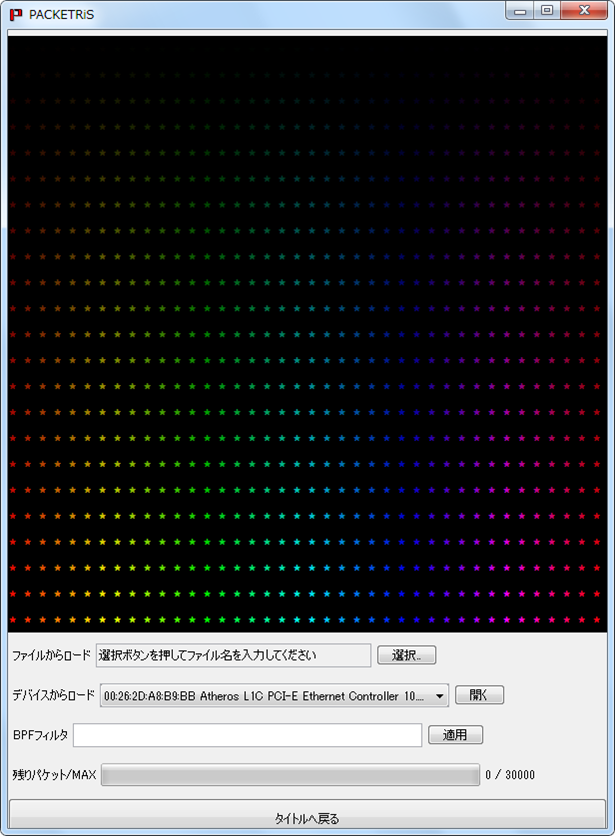
\includegraphics[width=9cm]{packetanalyze.png}
\caption{パケット解析機}
\end{figure}

\subsection{あたらしいパケットの保持}
制限付きのキューを作成し、到着したパケットを次々とキューに装填することで、
 新鮮なパケットを使うようにしている。

\subsection{完全なイベントドリブンへの拡張}
パケットの到着とそのプロトコルに即座に反応する独自のハンドラを用意し、
「デバイスからロード」を行った場合、完全にリアルタイムなプロトコルデータの抽出を、 簡単に実装できるようにした。これはパケットアート以外にも流用可能である。

\subsection{省メモリ性}
パケットを一時的に保持することはメモリの浪費に直結するが、
JNI(Java Native Interface)のライブラリが保持するオンメモリのデータへのポインタを
 一つしか持ち得ないクラスを作成し、使いまわすことでメモリの浪費を避けている。

\subsection{データに特化した開発}
WIDEプロジェクトではL3以上のレイヤがデータの肝となっているが、
 肝心のペイロードが除去されている。よって、必要以上の機能をつけることはやめ、
L3、L4を中心にした開発をした。


\section{ミノの生成方法について}
本作品はミノをパケットから生成している。その評価方法について以下に説明する。

\subsection{パケットの評価方法}
ミノの形状を生成するにあたり、まずパケットを一個、ロードする。
このパケットの読み込みは、デバイスまたはファイルからロードできる。
パケット不足を極力防ぐため、ある程度の数のパケットをプログラムの中で保持している。
次に、以下の表に基づいた情報を利用し、ミノを生成する。


\begin{table}[htbp]
\begin{center}
\caption{ミノの形状の決定表}
\begin{tabular}{|l|l|l|}
\hline
\multirow{3}{*}{IPv4} & TCP &シーケンス番号とチェックサム値 \\ \cline{2-3}
& UDP & 送信元ポート番号と宛先ポート番号 \\ \cline{2-3}
& その他 & IPIDシーケンス番号とチェックサム値 \\ \hline
\multirow{3}{*}{IPv6} & TCP & シーケンス番号とフラグフィールド \\ \cline{2-3}
& UDP & チェックサム値と宛先ポート番号  \\ \cline{2-3}
& その他 & フローラベルとデータペイロード長 \\ \hline
\multicolumn{2}{|l|}{その他} &  パケットサイズとミリ秒単位の時間 \\ \hline
\end{tabular}

\end{center}
\end{table}

このように複雑なのは、テトリミノの形が偏りすぎるのを防ぐためである。

次に、テトリミノ(4つのブロックが組となっているミノ)とペントミノ(5つのブロックが組となっているミノ)の両方がゲームに登場する設定の場合は
IPv4パケットを含むならばテトリミノを、それ以外はペントミノを テトリミノのブロックの数の決定因子にしている。
これも同様にバランスを考えてこのような条件にしている。

\section{ミノの描画方法について}
本作品は各ブロックに割り振られたパケットの情報を用いてミノのグラフィックを描画している。
描画がどのように行われているかについて、以下で説明する。

ミノの彩色においては、JavaにおけるHSB表色系の{\tt Color(H,S,B)}を使用する。
HSB表色系とは、色を色相(Hue)、彩度(Saturation)、輝度(Brightness)の三要素で表現する表色系である。
一般にコンピュータ上で用いられているRGBよりも「鮮やかな暗い赤」のように人間にとって直観的な色の表現が可能になる。
色相は一般的に円で表現され、色相環とも呼ばれる。

色相は変動で、ミノの持つパケットのチェックサムなどのパケットサイズを基軸からの回転量にした。
ミノ毎に色分けをするためである。紛らわしい色の重複を避けている。
彩度は固定で、1.0にした。これは鮮やかさを高くすることでミノの視認性を高くする目的である。。
輝度は変動で、ミノの持つパケットの最上階のレイヤが、OSI参照モデルにおいて、低いほど暗い色になる。

本作品ではオプションからミノに対して特定の文字を表示できる機能がある。この文字を決定する方法として以下の表を用いる。
この表は、ミノの描画に用いるパケットが''TCP over IPv4''のとき、「黄色のT」が表示される、と読む。

\begin{table}[htbp]
\begin{center}
\caption{色の決定テーブル}
\begin{tabular}{|l|l|l|l|l|l|}
\hline
 & TCP & UDP & ICMP & IPv4 & IPv6 \\ \hline \hline
IPv4 & 黄色のT & 緑のU & シアンのI & マゼンタの4 & 赤の6 \\ \hline
IPv6 & 青のT & 青のU & 白のI & 青の4 & 青の6 \\ \hline
Ethernet & 赤のT & 赤のU & 白のI & 白の4 & 白の6 \\ \hline
PPP & 赤のT & 赤のU & 白のI & 白の4 & 白の6 \\ \hline
その他 & 赤のT & 赤のU & 白のI & 白の4 & 白の6 \\ \hline
\end{tabular}
\end{center}
\end{table}

\begin{table}[htbp]
\begin{center}
\begin{tabular}{|l|l|}
\hline
プロトコル名 & 色と文字 \\ \hline \hline
 L2TP & 朱のL \\ \hline
 PPP & 朱のP \\ \hline
 ARP & 朱のA \\ \hline
 Ethernet & 朱のE \\ \hline
 OTHER & 朱の! \\ \hline
\end{tabular}
\end{center}
\end{table}

\begin{figure}[htbp]
\centering
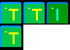
\includegraphics[width=5cm]{mino.png}
\caption{生成されるミノの例}
\end{figure}

\section{パケット情報からの自動作曲について}
本作品はパケットから音楽を自動で生成する機能が備わっており、パケットから自動生成された音楽をBGMにして、ゲームをプレイすることができる。
音楽を自動生成する場合、ただただ音符を無造作に並べただけではただの不協和音になる。
そこで、音楽理論に基づいた処理を行い、耳の心地よい音楽を生成するようになっている。

\subsection{自動作曲法について}
主旋律はIPv4の値から自動生成している。
IPv4の1オクテットから1/2小節を生成する。
伴奏は明暗2通りから固定で生成する。コード進行は固定である。
主旋律は自動生成とは言え、伴奏と不協和音にならない程度に範囲を縛っている。
ただ単にパケットの数字を音高に変換したものは、不協和音となってしまう可能性が非常に高く、音楽とは呼べない。

一般的に音楽は芸術的感性が重視されるように思われているかもしれないが、一種の規則性を持っており、それらは数学的に表すことができる。
つまり、パケットのもつ数字などから協和音的な音楽を生成することは可能である。
通常音楽にはコード進行があり、そのコード1つ1つにはそれぞれ適する音がいくつか存在する。
そこで予めコード進行は決めておき、そのコードに合う音をパケットの数字を基にして当てはめる。

これにより使用するパケットによって毎回違う音楽が生成される。

\begin{figure}[htbp]
\centering
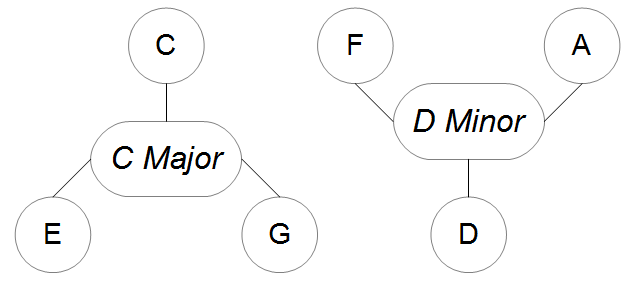
\includegraphics[width=10cm]{chord.png}
\caption{音楽の自動生成に用いるコード}
\end{figure}

\subsection{音楽の自動生成に関わるクラスについて}
音楽の自動生成に関わるクラスとその役割について以下に示す。

\begin{itemize}
\item CodeMaker

 BGMのコード進行を定義するクラスである。
 後々のBGM生成に大きな影響を与える。
このコード進行は自動生成ではなく、予め定義されたものとなっている。


\item ScaleMaker

 BGM生成に使用する鍵盤を定義するクラスである。
 不協和音を生成しないためには、正しい音階を用いて音楽を生成する必要がある。
 鍵盤には幹音(白鍵)と派生音(黒鍵)が同時に存在し、Javaでは低音から両者関係無く数字が順に割り振られている。
 長調と短調では一定の規則性で幹音と派生音の順番が決まっており、その規則性に従って使用する鍵盤を定義している。


\item MelodyAlgorithm

ロードしたパケット中からIPv4を取り出して処理し、主旋律の決定要素を作成するクラスである。
IPv4アドレスをオクテット毎に取り出し、その数値の大きさによって判定要素Aを確定させている。
また、ScaleMakerで定義したコードの協和音となる任意の音を定義し、これを判定要素Bとしている。
 以上の判定要素Aと判定要素Bを組み合わせて算出されたものが、音楽の主旋律の決定要素となる。


\item MelodyMaker

 BGMの主旋律を作成するクラスである。
BGMの1小節は4拍で構成されており、うち2拍をMelodyAlgorithmの主旋律の決定要素1つを用いて生成する。
ただ、それだけだと単調な音楽になってしまうため、偶数拍は先の決定要素の音を、奇数拍はそれを変化させた音を使用する。
この部分がパケットを基にしたBGMの自動生成要素となっている。


\item AccompanimentMaker

 BGMの伴奏を生成するクラスである。
 伴奏は自動生成ではなく、ScaleMakerで定義したコード進行に合う伴奏が予め定義されている。


\item MusicPlayer

自動生成したBGMを再生するクラスである。
MelodyMakerとAccompanimentMakerで生成されたBGMデータ(sequence)を組み合わせ、再生する。


\item MidiPlayer

外部Midiファイルを読み込み、再生するクラスである。
Midiファイルを一度開き、音量情報を指定のものに全て書き換え、出力再生する。

\end{itemize}

\section{システムについて}
本作品はJavaによって構成されている。特に、JavaのAWTとSwingを活用して、複数の画面を制御している。画面の制御などに関してはパケットに関する処理を行っていないため、詳細は割愛する。
本作品のソースコードは、Github\footnote{Github:\url{http://github.com/kobasemi/PacketArt}}で共有されている。また、本作品のソースコードはMIT Licenseとする。

本作品は起動時に複数のファイル読み込みが発生するため、その読み込み待ち時間にスプラッシュスクリーンを表示するようにしている。
そうすることでこの作品に触れる人が、ファイルの待ち時間に感じるストレスを小さくする狙いがある。

本作品はパケットからミノを生成するが、テトリミノの場合、7種類しか存在しない。そのため、ペントミノを生成できるようにし、12種類のミノを生成できるようにした。
また、テトリミノとペントミノを同時に出現できるようにすることで、19種類のミノを発生できるようにする。
そのため、難易度はテトリミノのみ、ペントミノのみ、テトリミノとペントミノの混合と3種類に分けることができる。

\section{本作品の開発手法}
本作品は1月ごろに作品の草案となる「パケット」と「テトリス」の組み合わせについて議論した。
本作品のプログラムの開発には、Processing\footnote{Processing:\url{http://processing.org/}}やC++、Javaが候補に挙がった。その中でプログラムの開発においてメモリリークなどの追跡困難なバグが発生しにくく、高い拡張性と、優秀なパケット読み込みライブラリが存在しており、開発コストと学習コストを鑑みた結果、
Javaを用いることになった。Javaを用いるうえで、パケットキャプチャリングを行うためのライブラリとしてJnetPcapを使用している。

本作品の開発に着手した時期は2月である。2月は大学の春季休業期間中であるため、開発メンバーで集まって開発することは難しいと判断したため、Githubを用いてソースコードの共有を行った。
本システムの設計にはUML(Unified Modeling Language)のクラス図やシーケンス図を用いており、オブジェクト指向の強いプログラムになっている。

本作品はvim、Eclipse、IntelliJ IDEAなどのいろいろなIDE(Integrated Development Environment)や、Windows、Linux、Macなどの多様な環境での開発が行われていた。

\begin{thebibliography}{99}
\bibitem{jnetpcap}{JnetPcap Documentation,\url{http://jnetpcap.com/jnetpcap-1.3} ,2013年5月18日確認}
\end{thebibliography}

\end{document}